\documentclass[11pt, a4paperm, hidelinks]{article}
\usepackage[utf8]{inputenc}
\usepackage[T1]{fontenc}
\usepackage[english]{babel}
\usepackage{lmodern}


\usepackage[a4paper,top=3cm,bottom=3cm,left=3cm,right=3cm]{geometry}
\usepackage{chngcntr}

%package used to enumerate figures
\usepackage[labelfont=bf]{caption}

%hyperref for interactive PDF index
\usepackage[bookmarks, colorlinks, breaklinks]{hyperref}
\hypersetup{linkcolor=black, citecolor=black, filecolor=black, urlcolor=black}

%Package required to use special symbols
\usepackage{amsmath, amssymb}

%Package required to use figures
\usepackage{graphicx}
\usepackage{subfig}
\usepackage{placeins}
\usepackage{wrapfig}

%Include the bibliography in the table of contents
\usepackage{tocbibind}

%Package used to insert figures at the specified position
\usepackage{float}
\usepackage{longtable}

\usepackage{times}

%Our chapters must be called sections
\addto\captionsenglish{\renewcommand{\chaptername}{Section}}

%Tables
\usepackage{hyperref}
\usepackage{graphicx}
\usepackage{caption}
\usepackage{booktabs}

%Header
\usepackage{fancyhdr}
\pagestyle{fancy}
\fancyhf{}
\rhead{Stefano Bagarin - Alessandra Pasini}
\lhead{User Testing Document}
\rfoot{Page \thepage}

\usepackage{xurl}
\begin{document}

	%Code for title page
	\begin{titlepage}
		\centering
		
\includegraphics[width=0.20\textwidth]{./assets/polimi-logo.png}\par

		{Politecnico di Milano \\ AA 2019/2020} \par
		\vspace{1.5cm}

		{Computer Science and Engineering}\par
		\Large{Hypermidia Applications}\par
		\vspace{1.0cm}

		{\LARGE \textbf{User Testing Document} \par}
		\vspace{1.5cm}

		{\normalsize {\textbf{Stefano Bagarin}: mrt. 945159 -  stefano.bagarin@mail.polimi.it }\par}
		\vspace{0.2cm}
		{\normalsize{\textbf{Alessandra Pasini}: mtr. 920051 - alessandra.pasini@mail.polimi.it}\par}
		\vspace{1.0cm}
		
		{\normalsize {\textbf{Our website}: \url{https://wild-care.herokuapp.com/index.html}}\par}
		\vspace{0.2cm}
		{\normalsize {\textbf{Delivery final date}: July 6, 2020}\par}
		\vfill

		% Bottom of the page
		{\large Document version: 1.0\par}
		{\large \today \par}
	\end{titlepage}

	%Make the table of contents
	\tableofcontents
	\clearpage


	%Abstract
	\section{Abstract}
	The aim of this document is to report the User-Testing-based Usability Evaluation of Wild Care website which can be found at 	\url{https://wild-care.herokuapp.com/}.	\\ The website that is analyzed into this document is intended to provide 				information about Wild Care association, the events that it organizes, the services provided and the volunteers that are 			involved into the association and its activities. It also gives the possibility to read faqs and to sent request via a form.\\
 	Tester followed a 2 steps procedure:
	\begin{enumerate}
		\item Execute given task following scenarios while they are evaluated with specific criteria
		\item Surf the website freely
		\item Fulfill a form with some questions related to landmarks, navigation and layout.
	\end{enumerate}	

	%Design
	\section{Design of the study}
	\subsection{User profile definition}
We have defined 2 segments of user profiles heterogeneous for what concern the gender and homogeneous for what concern 	other age, civil state and tech capabilities.
\begin{itemize}
		\item \textbf{User profile one}
			\begin{itemize}
				\item \emph{Age range}: between 18 to 35 years old
				\item \emph{Civil State}: single or with fiancee
				\item \emph{Technology capabilities}: normal web user with no peculiar capabilities
			\end{itemize}
		\item \textbf{User profile two}
			\begin{itemize}
				\item \emph{Age range}: between 40 to 60 years old
				\item \emph{Civil State}: merried
				\item \emph{Technology capabilities}: normal web user with no peculiar capabilities
			\end{itemize}
\end{itemize}


\subsection{Scenarios}
The User testing is based on 3 scenarios
\begin{itemize}
		\item \textbf{Scenario 1}\\ You are planning to go to Valtellina in September and you are looking for an event related to 				wild animals; once you get it you wanna know more and decide to call the event organizer.
			\begin{enumerate}
				\item Surf the events and find the Septemeber ones
				\item Select an event that you like
				\item Find even organizer phone number to contact him/her and get more info
			\end{enumerate}
		\item \textbf{Scenario 2}\\ You would like to become volunteer of an association that protects wild animals.
			\begin{enumerate}
				\item Get info about the association
				\item Try to answer to your question reading faqs
				\item Send a request to become volunteer
			\end{enumerate}
		\item \textbf{Scenario 3}\\ You are discovering Wild Care services and you would like to get more information about the 			event related to a certain service that you liked the most.
			\begin{enumerate}
				\item Surf the services
				\item Select a service that you find interesting 
				\item Pick a related event and see its details
			\end{enumerate}
\end{itemize}

\subsection{Variables to measure}
To evaluate the task execution we have chosen to adopt the following metrics:
\begin{itemize}
	\item \emph{time of execution}: the clock starts when the user directs his/her attention to the application
	\item \emph{success rate}: to a "complete success" is assigned a value equal to 1, to a "partial success" is assigned a value 		equal to 0.5 and to a "failure" a value equal to 0.0
	\item \emph{perceived difficulty}: an oral evaluation between 0 and 5 given imemediately after the task execution
	\item \emph{errors}: integer that express how many "wrong" links have been clicked to reach the goal or wrong paths have 		been taken
	\item \emph{satisfaction}: an oral evaluation between 0 and 5 given imemediately after the task execution
\end{itemize}

\subsection{Final survey}
After all tasks execution, every user fulfilled a questionnaire formed by N questions with a rating between 0 to 5. We have used Forms Pro software to create the survey and collect data; we have reported here all questions for completeness.
\begin{enumerate}
	\item How much useful did you find the topbar? 
	\item How much easy has it been to find events for month?
	\item How much easy has it been to find services related to events?
	\item How much easy has it been to find events organized by a volunteer?
	\item How much easy has it been to find volunteer's details?
	\item How easily did you find the mission of the association?
	\item Do you find the text layout readable?
	\item Do you find images dimension good?
	\item Do you find website layout consistent?
	\item Are semantic close events also close into the space?
\end{enumerate}
The survey can be found at link \\ \url{https://forms.office.com/FormsPro/Pages/ResponsePage.aspx?id=8eAiizYZfk-CTpheWGbGkZgSwAPI3GJPvXJ0APwN3yxUNU42NjFRRTIwTlA5SENQWTNKVEwwQzRBTS4u}.



	%Execution
	\section{Execution of the study}
	The study has been executed in person at the end of the development of the website. The testers used their own laptop or our while we manually gather usability data. We took two tests at a time in parallel to reduce time and make it faster. In order to be sure that every tester didn't see the website before the execution we divided them in different rooms, who was doing the test was in one room with one of the developers and the others where waiting in the living room.\\ We have also chosen to respect our tester privacy and, for this reason, they are represented here through IDs.

\subsection{User Profile 1}
Here it is possible to see the result of task execution of each user belonging to user profile 1.
{\centering
\captionof{table}{Evaluation tester ID 0000}
\centering
\begin{tabular}{lllllll} 
	\toprule
	\textbf{Scenario } & \textbf{Task} & \begin{tabular}[c]{@{}l@{}}\textbf{Execution}\\\textbf{Time (s)}\end{tabular} & \textbf{Success} & \begin{tabular}[c]{@{}l@{}}\textbf{Perceived}\\\textbf{Difficulty}\end{tabular} & \textbf{Errors} & \textbf{Satisfaction}  \\
	Scenario 1 & 1             & 10                 & 1.0          & 0                                                                          & 0					& 5           	                                                                 \\
	Scenario 1 & 2             & 5                   & 1.0          & 0                                                                          & 0					& 5                                                                                \\
	Scenario 1 & 3             & 10                 & 1.0          & 0                                                                          & 0					& 5                                                                                \\
	Scenario 2 & 1             & 11                 & 1.0          & 0                                                                          & 0					& 4                                                                                \\
	Scenario 2 & 2             & 6                   & 1.0          & 0                                                                          & 0					& 5                                                                                \\
	Scenario 2 & 3             & 37                 & 1.0          & 1                                                                          & 2					& 4                                                                                \\
	Scenario 3 & 1             & 10                 & 1.0          & 0                                                                          & 0					& 4                                                                                \\
	Scenario 3 & 2             & 12                 & 1.0          & 0                                                                          & 0					& 4                                                                                \\
	Scenario 3 & 3             & 24                 & 1.0          & 0                                                                          & 0					& 4                                                                                 \\
	\bottomrule
\end{tabular}

\vspace{1cm}


\centering
\captionof{table}{Evaluation tester ID 0002}
\centering
\begin{tabular}{lllllll} 
	\toprule
	\textbf{Scenario } & \textbf{Task} & \begin{tabular}[c]{@{}l@{}}\textbf{Execution}\\\textbf{Time (s)}\end{tabular} & \textbf{Success} & \begin{tabular}[c]{@{}l@{}}\textbf{Perceived}\\\textbf{Difficulty}\end{tabular} & \textbf{Errors} & \textbf{Satisfaction}  \\
	Scenario 1 & 1             & 10                 & 1.0          & 0                                                                          & 0					& 4           	                                                                 \\
	Scenario 1 & 2             & 20                 & 1.0          & 0                                                                          & 0					& 5                                                                                \\
	Scenario 1 & 3             & 40                 & 1.0          & 1                                                                          & 0					& 4                                                                                \\
	Scenario 2 & 1             & 25                 & 1.0          & 0                                                                          & 0					& 5                                                                                \\
	Scenario 2 & 2             & 20                 & 1.0          & 0                                                                          & 0					& 4                                                                                \\
	Scenario 2 & 3             & 90                 & 1.0          & 0                                                                          & 0					& 5                                                                                \\
	Scenario 3 & 1             & 30                 & 1.0          & 0                                                                          & 0					& 4                                                                                \\
	Scenario 3 & 2             & 40                 & 1.0          & 0                                                                          & 0					& 5
\\
	Scenario 3 & 3             & 60                 & 1.0          & 1                                                                          & 0					& 5                                                                                 \\
	\bottomrule
\end{tabular}

\vspace{1cm}

\centering
\captionof{table}{Evaluation tester 0003}
\centering
\begin{tabular}{lllllll} 
	\toprule
	\textbf{Scenario } & \textbf{Task} & \begin{tabular}[c]{@{}l@{}}\textbf{Execution}\\\textbf{Time (s)}\end{tabular} & \textbf{Success} & \begin{tabular}[c]{@{}l@{}}\textbf{Perceived}\\\textbf{Difficulty}\end{tabular} & \textbf{Errors} & \textbf{Satisfaction}  \\
	Scenario 1 & 1             & 20                 & 1.0          & 0                                                                          & 0					& 5           	                                                                 \\
	Scenario 1 & 2             & 20                 & 1.0          & 0                                                                          & 0					& 5                                                                                \\
	Scenario 1 & 3             & 40                 & 1.0            & 0                                                                          & 0					& 5                                                                                \\
	Scenario 2 & 1             & 25                 & 1.0          & 0                                                                          & 0					& 5                                                                                \\
	Scenario 2 & 2             & 20                 & 1.0          & 1                                                                          & 0					& 5                                                                                \\
	Scenario 2 & 3             & 90                 & 1.0          & 0                                                                          & 0					& 5                                                                                \\
	Scenario 3 & 1             & 30                 & 1.0          & 0                                                                          & 0					& 5                                                                                \\
	Scenario 3 & 2             & 40                 & 1.0          & 0                                                                          & 0					& 5                                                                                \\
	Scenario 3 & 3             & 60                 & 1.0          & 0                                                                          & 0					& 5                                                                                 \\
	\bottomrule
\end{tabular}

\vspace{1cm}


\centering
\captionof{table}{Evaluation tester 0007}
\centering
\begin{tabular}{lllllll} 
	\toprule
	\textbf{Scenario } & \textbf{Task} & \begin{tabular}[c]{@{}l@{}}\textbf{Execution}\\\textbf{Time}\end{tabular} & \textbf{Success} & \begin{tabular}[c]{@{}l@{}}\textbf{Perceived}\\\textbf{Difficulty}\end{tabular} & \textbf{Errors} & \textbf{Satisfaction}  \\
	Scenario 1 & 1             & 9                 & 1.0          & 0                                                                          & 0					& 5           	                                                                 \\
	Scenario 1 & 2             & 5                 & 1.0          & 0                                                                          & 0					& 5                                                                                \\
	Scenario 1 & 3             & 15                 & 1.0            & 0                                                                          & 1					& 5                                                                                \\
	Scenario 2 & 1             & 10                 & 1.0          & 0                                                                          & 0					& 5                                                                                \\
	Scenario 2 & 2             & 40                 & 1.0          & 1                                                                          & 1					& 5                                                                                \\
	Scenario 2 & 3             & 55                 & 1.0          & 0                                                                          & 1					& 5                                                                                \\
	Scenario 3 & 1             & 4                 & 1.0          & 0                                                                          & 0					& 5                                                                                \\
	Scenario 3 & 2             & 10                 & 1.0          & 0                                                                          & 0					& 5                                                                                \\
	Scenario 3 & 3             & 15                 & 1.0          & 0                                                                          & 0					& 5                                                                                 \\
	\bottomrule
\end{tabular}

\vspace{1cm}


\centering
\captionof{table}{Evaluation tester 0008}
\centering
\begin{tabular}{lllllll} 
	\toprule
	\textbf{Scenario } & \textbf{Task} & \begin{tabular}[c]{@{}l@{}}\textbf{Execution}\\\textbf{Time}\end{tabular} & \textbf{Success} & \begin{tabular}[c]{@{}l@{}}\textbf{Perceived}\\\textbf{Difficulty}\end{tabular} & \textbf{Errors} & \textbf{Satisfaction}  \\
	Scenario 1 & 1             & 10                 & 1.0          & 0                                                                          & 0					& 5           	                                                                 \\
	Scenario 1 & 2             & 21                 & 1.0          & 0                                                                          & 0					& 5                                                                                \\
	Scenario 1 & 3             & 20                 & 1.0            & 0                                                                          & 0					& 5                                                                                \\
	Scenario 2 & 1             & 6                 & 1.0          & 1                                                                          & 1					& 4                                                                                \\
	Scenario 2 & 2             & 88                 & 1.0          & 3                                                                          & 0					& 5                                                                                \\
	Scenario 2 & 3             & 91                 & 1.0          & 0                                                                          & 0					& 5                                                                                \\
	Scenario 3 & 1             & 4                 & 1.0          & 0                                                                          & 0					& 5                                                                                \\
	Scenario 3 & 2             & 10                 & 1.0          & 0                                                                          & 0					& 5                                                                                \\
	Scenario 3 & 3             & 20                 & 1.0          & 1                                                                          & 1					& 4                                                                                 \\
	\bottomrule
\end{tabular}

\vspace{1cm}
}

\subsection{User Profile 2}
Here it is possible to see the result of task execution of each user belonging to user profile 2. \\ They got some problems when they had to find the phone number of a volunteer that organized a certain event \emph{(Scenario 1: task 3)} and the errors they made where given by the fact that they where searching this kind of information into "About us" page or by going to "All People" without remembering the organizer's name. They suggested to put organizers info upper into the "Event" page or add contact info directly to the "Event" page.

{
\captionof{table}{Evaluation tester ID 0001}
\centering
\begin{tabular}{lllllll} 
	\toprule
	\textbf{Scenario } & \textbf{Task} & \begin{tabular}[c]{@{}l@{}}\textbf{Execution}\\\textbf{Time (s)}\end{tabular} & \textbf{Success} & \begin{tabular}[c]{@{}l@{}}\textbf{Perceived}\\\textbf{Difficulty}\end{tabular} & \textbf{Errors} & \textbf{Satisfaction}  \\
	Scenario 1 & 1             & 13                 & 1.0          & 0                                                                          & 0					& 5           	                                                                 \\
	Scenario 1 & 2             & 7                & 1.0          & 0                                                                          & 0					& 5                                                                                \\
	Scenario 1 & 3             & 18                 & 1.0          & 2                                                                          & 2					& 3                                                                                \\
	Scenario 2 & 1             & 6                 & 1.0          & 0                                                                          & 0					& 5                                                                                \\
	Scenario 2 & 2             & 11                 & 1.0          & 0                                                                          & 0					& 5                                                                                \\
	Scenario 2 & 3             & 12                 & 1.0          & 0                                                                          & 0					& 5                                                                                \\
	Scenario 3 & 1             & 15                 & 1.0          & 0                                                                          & 0					& 5                                                                                \\
	Scenario 3 & 2             & 17                 & 1.0          & 0                                                                          & 0					& 5                                                                                \\
	Scenario 3 & 3             & 12                 & 1.0          & 1                                                                          & 0					& 4                                                                                 \\
	\bottomrule
\end{tabular}

\vspace{1cm}

\centering
\captionof{table}{Evaluation tester ID 0004}
\centering
\begin{tabular}{lllllll} 
	\toprule
	\textbf{Scenario } & \textbf{Task} & \begin{tabular}[c]{@{}l@{}}\textbf{Execution}\\\textbf{Time (s)}\end{tabular} & \textbf{Success} & \begin{tabular}[c]{@{}l@{}}\textbf{Perceived}\\\textbf{Difficulty}\end{tabular} & \textbf{Errors} & \textbf{Satisfaction}  \\
	Scenario 1 & 1             & 13                 & 1.0          & 0                                                                          & 0					& 5           	                                                                 \\
	Scenario 1 & 2             & 9               & 1.0          & 0                                                                          & 0					& 5                                                                                \\
	Scenario 1 & 3             & 15                 & 1.0          & 1                                                                          & 1				& 4                                                                                \\
	Scenario 2 & 1             & 25                 & 1.0          & 1                                                                          & 1					& 4                                                                                \\
	Scenario 2 & 2             & 7                 & 1.0          & 0                                                                          & 0					& 5                                                                                \\
	Scenario 2 & 3             & 18                 & 1.0          & 0                                                                          & 0					& 5                                                                                \\
	Scenario 3 & 1             & 11                & 1.0          & 0                                                                          & 0					& 5                                                                                \\
	Scenario 3 & 2             & 4                 & 1.0          & 0                                                                          & 0					& 5                                                                                \\
	Scenario 3 & 3             & 10                 & 1.0          & 0                                                                          & 0					& 5                                                                                \\
	\bottomrule
\end{tabular}

\vspace{1cm}

\centering
\captionof{table}{Evaluation tester ID 0005}
\centering
\begin{tabular}{lllllll} 
	\toprule
	\textbf{Scenario } & \textbf{Task} & \begin{tabular}[c]{@{}l@{}}\textbf{Execution}\\\textbf{Time (s)}\end{tabular} & \textbf{Success} & \begin{tabular}[c]{@{}l@{}}\textbf{Perceived}\\\textbf{Difficulty}\end{tabular} & \textbf{Errors} & \textbf{Satisfaction}  \\
	Scenario 1 & 1             & 21                 & 1.0          & 0                                                                          & 0					& 5           	                                                                 \\
	Scenario 1 & 2             & 12               & 1.0          & 0                                                                          & 0					& 5                                                                                \\
	Scenario 1 & 3             & 25                 & 1.0          & 2                                                                          & 2					& 4                                                                                \\
	Scenario 2 & 1             & 7                 & 1.0          & 0                                                                          & 0					& 5                                                                                \\
	Scenario 2 & 2             & 5                 & 1.0          & 0                                                                          & 0					& 5                                                                                \\
	Scenario 2 & 3             & 4                 & 1.0          & 0                                                                          & 0					& 5                                                                                \\
	Scenario 3 & 1             & 13                & 1.0          & 0                                                                          & 0					& 5                                                                                \\
	Scenario 3 & 2             & 20                 & 1.0          & 0                                                                          & 0					& 5                                                                                \\
	Scenario 3 & 3             & 21                 & 1.0          & 0                                                                          & 0					& 4                                                                                 \\
	\bottomrule
\end{tabular}

\vspace{1cm}

\centering
\captionof{table}{Evaluation tester ID 0006}
\centering
\begin{tabular}{lllllll} 
	\toprule
	\textbf{Scenario } & \textbf{Task} & \begin{tabular}[c]{@{}l@{}}\textbf{Execution}\\\textbf{Time (s)}\end{tabular} & \textbf{Success} & \begin{tabular}[c]{@{}l@{}}\textbf{Perceived}\\\textbf{Difficulty}\end{tabular} & \textbf{Errors} & \textbf{Satisfaction}  \\
	Scenario 1 & 1             & 14                 & 1.0          & 0                                                                          & 0					& 5           	                                                                 \\
	Scenario 1 & 2             & 4               & 1.0          & 0                                                                          & 0					& 5                                                                                \\
	Scenario 1 & 3             & 18                 & 1.0          & 1                                                                          & 2					& 4                                                                                \\
	Scenario 2 & 1             & 5                 & 1.0          & 0                                                                          & 0					& 5                                                                                \\
	Scenario 2 & 2             & 11                 & 1.0          & 0                                                                          & 0					& 5                                                                                \\
	Scenario 2 & 3             & 5                 & 1.0          & 0                                                                          & 0					& 5                                                                                \\
	Scenario 3 & 1             & 22                & 1.0          & 0                                                                          & 0					& 5                                                                                \\
	Scenario 3 & 2             & 19                 & 1.0          & 0                                                                          & 0					& 5                                                                                \\
	Scenario 3 & 3             & 15                 & 1.0          & 0                                                                          & 0					& 5                                                                                \\
	\bottomrule
\end{tabular}

\vspace{1cm}
}


	%Results
	\section{Results}
	This subsection shows the avg. of \emph{User Profile 1}'s results, the avg. of \emph{User Profile 2}'s results and the avg. between the two. We have chosen to give you also the separates view of the two groups to better understand how different segments react to the same tasks.

\subsection{Avg. User Profile 1}
{
\captionof{table}{Avg per task}
\centering
\begin{tabular}{lllllll} 
	\toprule
	\textbf{Scenario } & \textbf{Task} & \begin{tabular}[c]{@{}l@{}}\textbf{Execution}\\\textbf{Time (s)}\end{tabular} & 			\textbf{Success} & \begin{tabular}[c]{@{}l@{}}\textbf{Perceived}\\\textbf{Difficulty}\end{tabular} & \textbf{Errors} & 			\textbf{Satisfaction}  \\
	Scenario 1 & 1             & 9,4                 	& 100\%          	& 0					& 0					& 4,8           	                                                                 \\
	Scenario 1 & 2             & 8,6                   	& 100\%          	& 0					& 0					& 5                                                                                \\
	Scenario 1 & 3             & 15,2                 	& 100\%          	& 0,2				& 0,2				& 4,8                                                                               \\
	Scenario 2 & 1             & 8,8                 	& 100\%          	& 0,2				& 0,2				& 4,6                                                                              \\
	Scenario 2 & 2             & 36,4                   	& 100\%        	& 0					& 0,2				& 4,8                                                                                \\
	Scenario 2 & 3             & 46                 	& 100\%          	& 0,4				& 0,6				& 4,8                                                                                \\
	Scenario 3 & 1             & 8,2                 	& 100\%         	& 0					& 0					& 4,6                                                                                \\
	Scenario 3 & 2             & 11,2                 	& 100\%          	& 0					& 0					& 4,8                                                                                \\
	Scenario 3 & 3             & 18,6                	& 100\%          	& 0,4				& 0,2				& 4,6                                                                                 \\
\bottomrule
\end{tabular}

\vspace{1cm}
}It is possibile to see that, for this segment, the tasks 2 and 3 of scenario 2 has been the most complex and difficult and it can be seen becase the execution time is the heigher as the number of mistakes made and as the perceived difficulty. Even though the results into scenario 2 aren't that good, the satisfaction is high because they said that the problems they faced where related to the language. They suggested to add the multi-language feature in other to avoid the language barrier.\\
The next figure has the aim to show the avg between all scenarios.

\begin{figure}[h!]
	\centering
	\begin{minipage}[b]{1\textwidth}
    		
\includegraphics[width=\textwidth]{./assets/avg-1.png}
		\caption{\emph{Total Avg. user profile 1}: the avg obtained here is between the 3 scenarios }
	\end{minipage}
\end{figure}
\FloatBarrier


\subsection{Avg. User Profile 2}
{
\captionof{table}{Avg per task}
\centering
\begin{tabular}{lllllll} 
	\toprule
	\textbf{Scenario } & \textbf{Task} & \begin{tabular}[c]{@{}l@{}}\textbf{Execution}\\\textbf{Time (s)}\end{tabular} & 			\textbf{Success} & \begin{tabular}[c]{@{}l@{}}\textbf{Perceived}\\\textbf{Difficulty}\end{tabular} & \textbf{Errors} & 			\textbf{Satisfaction}  \\
	Scenario 1 & 1             & 15,25                 	& 100\%          	& 0					& 0					& 5           	                                                                 \\
	Scenario 1 & 2             & 8                   	& 100\%          	& 0					& 0					& 5                                                                                \\
	Scenario 1 & 3             & 19                 	& 100\%          	& 1,5				& 1,75				& 3,75                                                                               \\
	Scenario 2 & 1             & 10,75                 	& 100\%          	& 0,25				& 0,25				& 4,75                                                                              \\
	Scenario 2 & 2             & 8,5                   	& 100\%        	& 0					& 0					& 5                                                                                \\
	Scenario 2 & 3             & 9,75                 	& 100\%          	& 1					& 0,5				& 4                                                                                \\
	Scenario 3 & 1             & 15,25                 	& 100\%         	& 0					& 0					& 5                                                                                \\
	Scenario 3 & 2             & 15                 	& 100\%          	& 0					& 0					& 5                                                                                \\
	Scenario 3 & 3             & 14,5                	& 100\%          	& 0,25				& 0					& 4,5                                                                                 \\
\bottomrule
\end{tabular}

\vspace{1cm}
}It is possibile to see that for this segment the 3 task of scenario 1 has been the most complex and difficult and it can be seen becase the execution time is the heigher as the number of mistakes made and the satisfaction rate is the lower one. \\
The next figure has the aim to show the avg between all scenarios.

\begin{figure}[h!]
	\centering
	\begin{minipage}[b]{1\textwidth}
    		
\includegraphics[width=\textwidth]{./assets/avg-2.png}
		\caption{\emph{Total Avg. user profile 2}: the avg obtained here is between the 3 scenarios }
	\end{minipage}
\end{figure}
\FloatBarrier


\subsection{Total Avg.}
We have seen that there isn't a big difference between the results obtained by the 2 segments and we have also noticed that the avg of segment 2 is always higher than the avg obtain by segment 1 except for the satisfaction, which is lower. The next figure wrap up the results of the two,  in order to give a general final picture of scenarios. execution.
\begin{figure}[h!]
	\centering
	\begin{minipage}[b]{1\textwidth}
    		
\includegraphics[width=\textwidth]{./assets/avg-tot.png}
		\caption{\emph{Total Avg.}: the avg obtained here is between the 2 segments}
	\end{minipage}
\end{figure}
\FloatBarrier

\subsection{Survey results}
This section has the aim to show the avg result of each survey question and how the answers are divided between the different values.

\begin{figure}[h!]
	\centering
	\begin{minipage}[b]{1\textwidth}
    		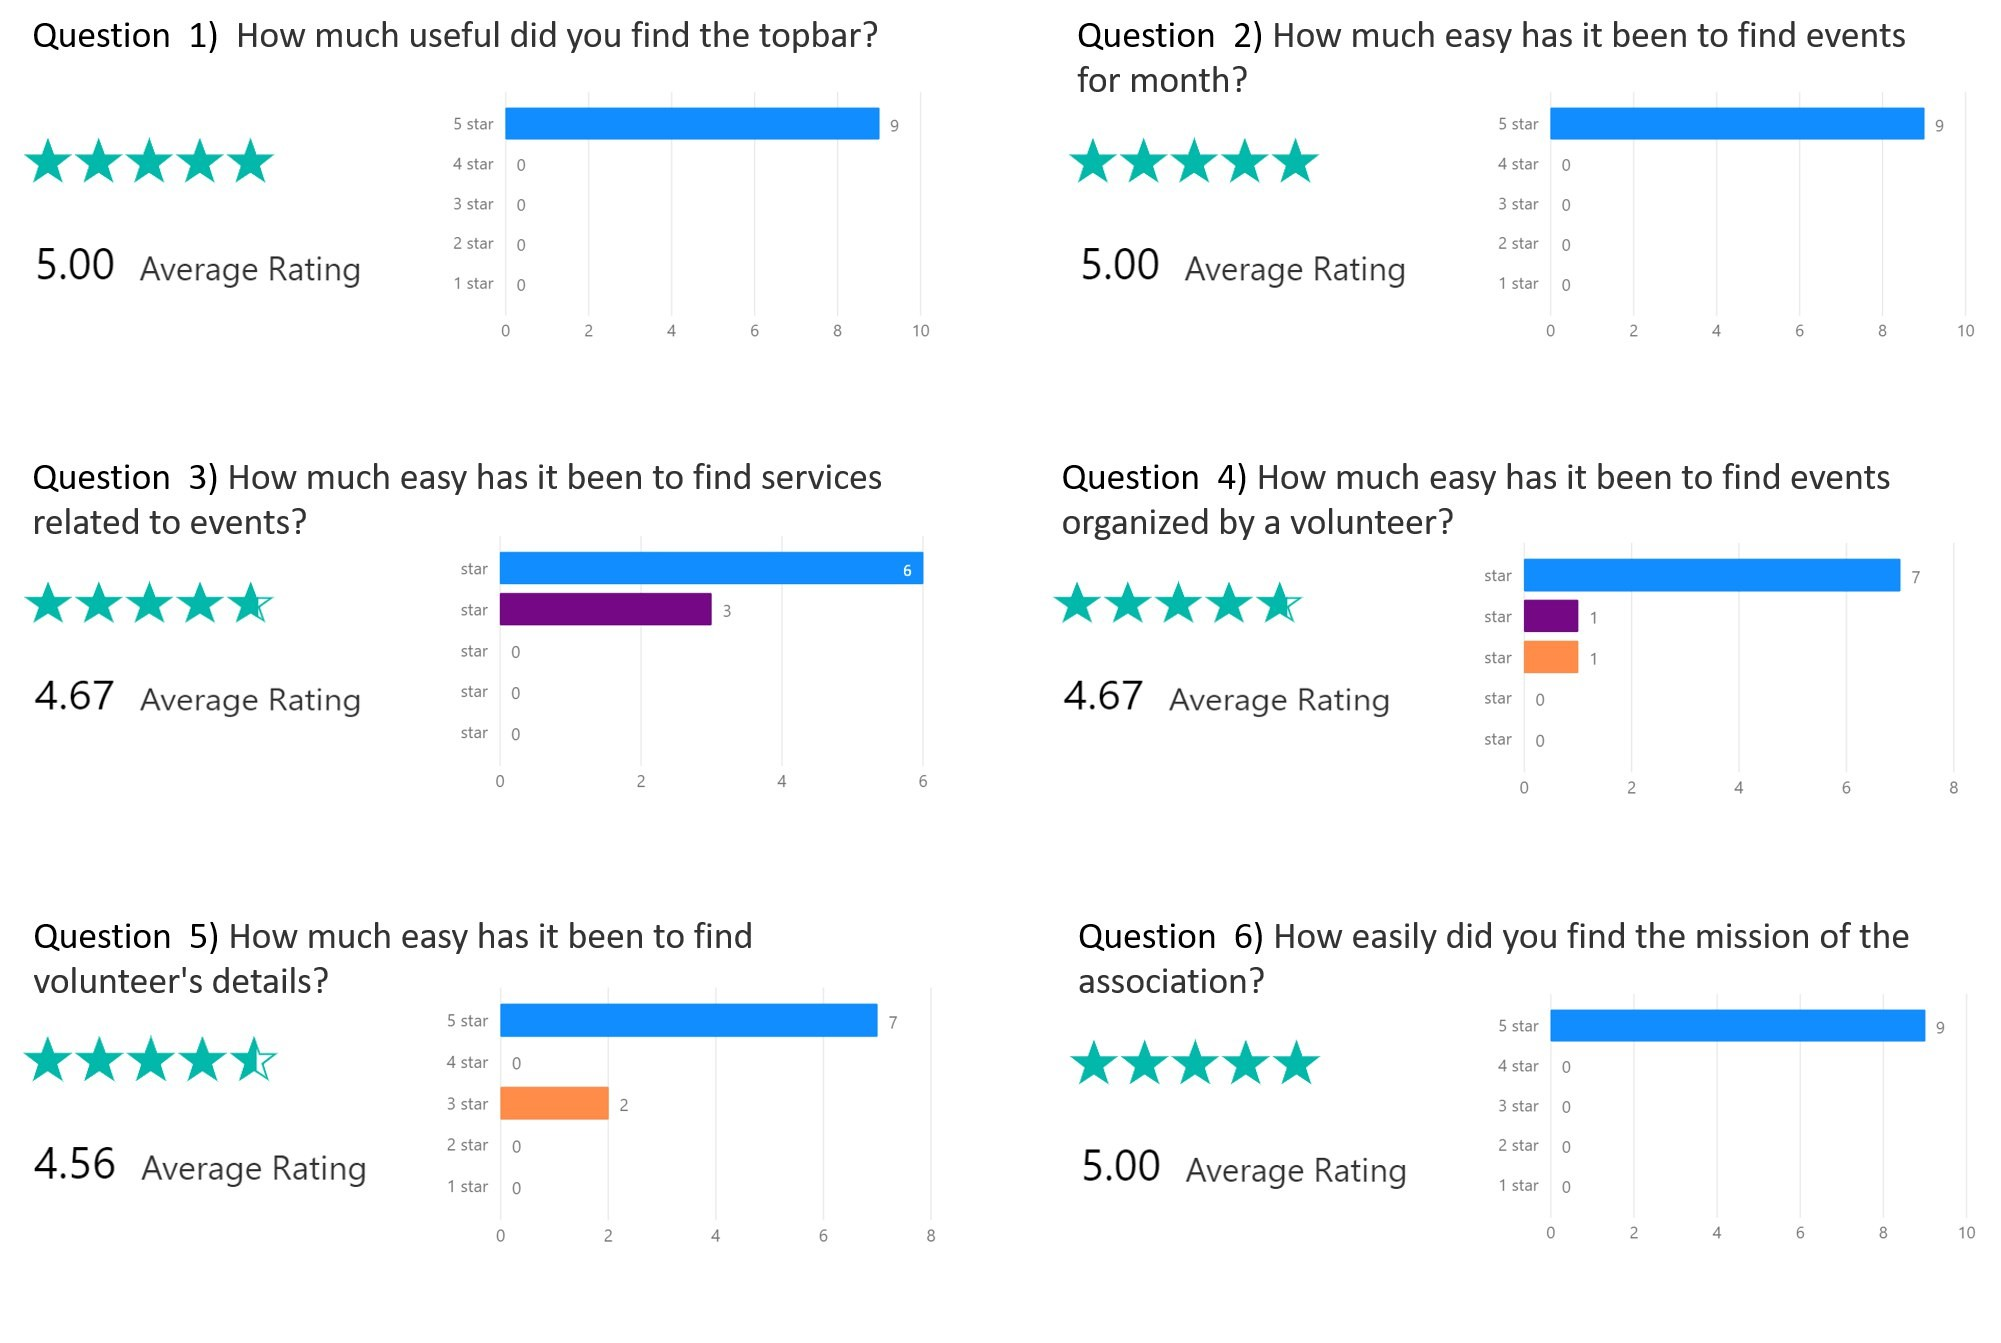
\includegraphics[width=\textwidth]{./assets/survey-results.jpg}
		\caption{Survey answers results}
	\end{minipage}
\end{figure}
\FloatBarrier
\begin{figure}[h!]
	\centering
	\begin{minipage}[b]{1\textwidth}
    		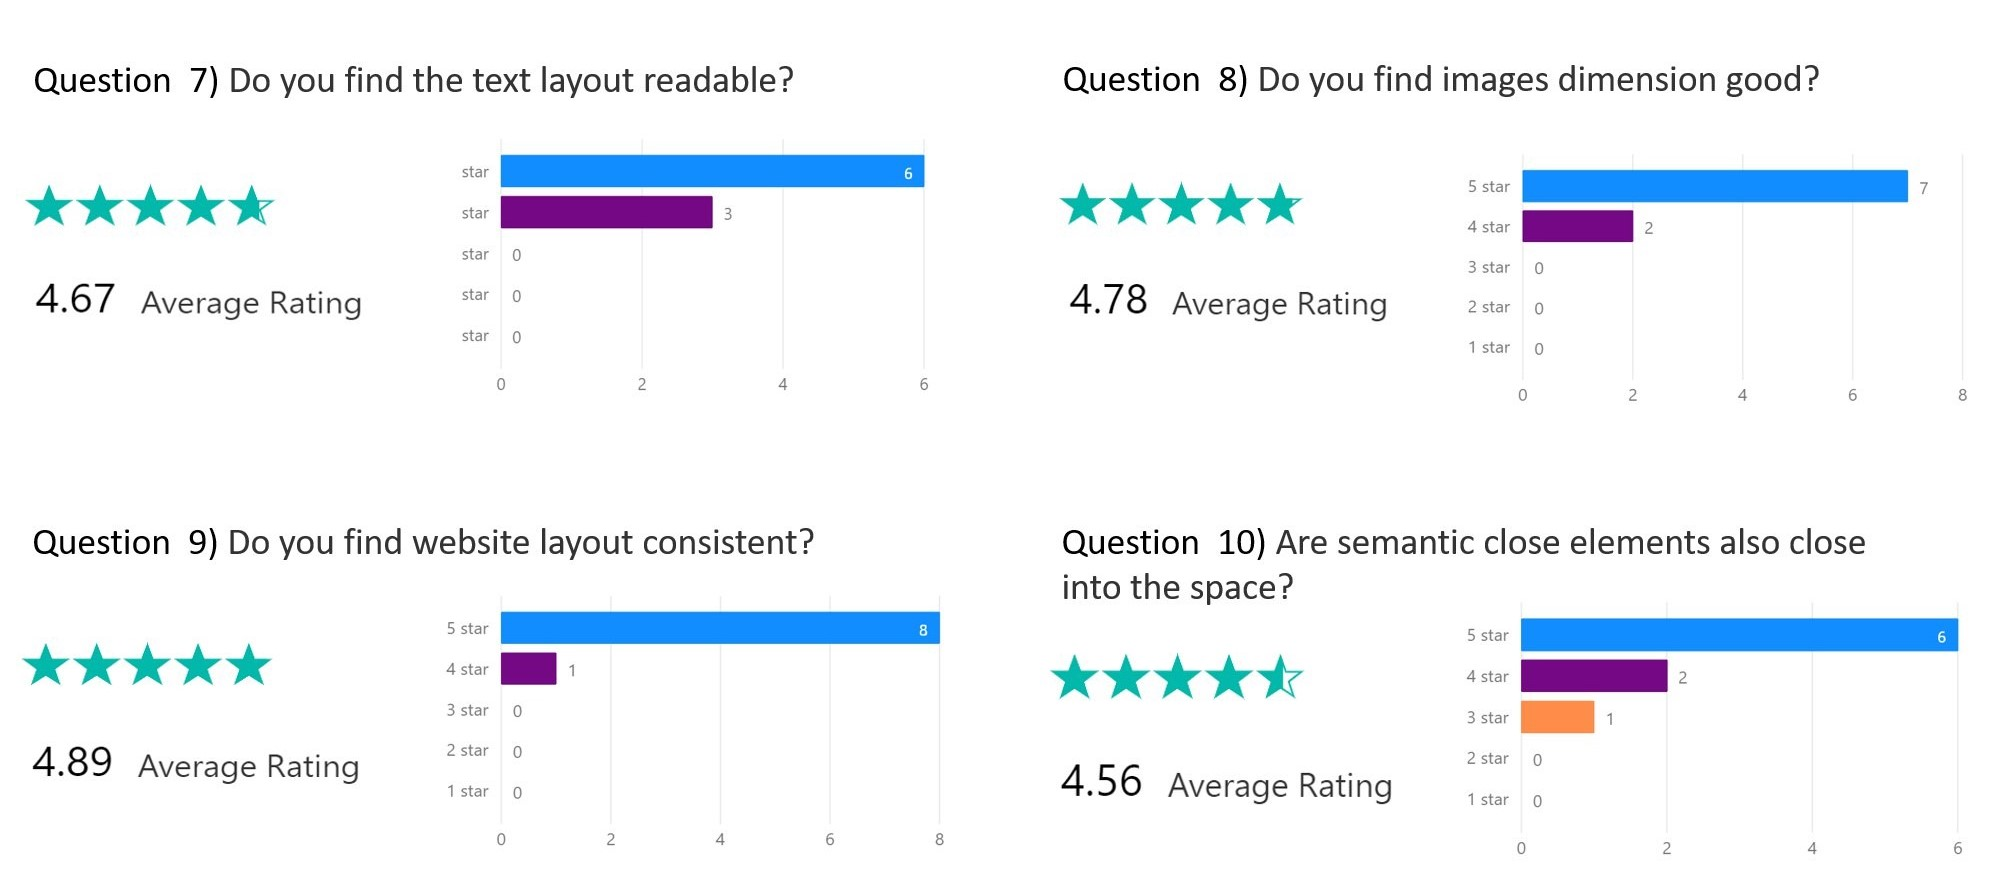
\includegraphics[width=\textwidth]{./assets/survey-results-1.jpg}
		\caption{Survey answers results}
	\end{minipage}
\end{figure}
\FloatBarrier

	\clearpage


	%Conclusion
	\section{Conclusion}	
	\clearpage

\end{document}
